\documentclass[dissertation,appendsingle,copyrightcc]{MSUstyle}
%
%  Created by Seth Humphries 
%  Update and maintained by Prof. Mark Owkes mark.owkes@montana.edu
% 
%%    Copyright (c) 2007-2012 Seth D. Humphries
%%    This work is licensed under the Creative Commons
%%    Attribution-Noncommercial-Share Alike 3.0 License. To view a copy
%%    of this license, visit http://creativecommons.org/licenses/by-nc-sa/3.0/;
%%    or, (b) send a letter to Creative Commons, 171 2nd Street, Suite
%%    300, San Francisco, California, 94105, USA. 
%
%  Version 2.0, check for periodic updates on the bitbucket repository
%
% DEFAULTS --------------------
% The default options are as follows:
%   \documentclass[12pt,letterpaper,oneside,openright,%
%       doublespaced,normalmargins,dissertation,final,numreset]{MSUstyle}
%
% default options do not need to be entered. Defaults will generate a document 
% that conforms to the MSU Electronic Thesis/Dissertation  (ETD) guidelines. 
%
% MASTERS THESIS ---------------
%  use \documentclass[thesis]{MSUstyle} to adjustment the front matter according to ETD style rules that
% are different for a thesis than for a dissertation.
%
% COMPREHENSIVE EXAM -----------
% \use \documenatclass[compexam]{MSUstyle} to format the document for a written
% comprehensive exam. This only changes "dissertation" to "comprehensive exam";
% everything else is the same as the dissertation format. This is an acceptable
% format for the written comprehensive exam in the Electrical and Computer
% Engineering department; other departments may vary.
%
% COPYRIGHT OPTIONS -----------
% If you want to license your work under a Creative Commons BY 4.0 license,
% use the copyrightcc option
%
% ADDITIONAL OPTIONS ----------
% 10pt, singlespaced, and draft allow you to require less number of pages for editing
% A draft version number can be set with, e.g., \draftver{1.0}
%
% numberedsections provides numbered chapter and section titles
%
% appendsingle/appendmultiple is required if you have one/multiple appendices, remove if you do not have an appendix
%
% nonumreset does not add chapter to labels of figures, tables, etc. (not recommended)
%
% PRINTING OPTIONS ------------
% oneside,openright (defaults) 1" margin on all sides of pages (use for electronic documents and submission to grad school)
% oneside,openright,bigmargin larger margin on left side of pages (optionally use for electronic documents and submission to grad school)
% twoside,openright  1" margins,  blank pages added so chapter start on right page (use for printing on minimal number of pages)
% twoside,openright,bigmargin larger margins alternate left/right sides for binding and ...
%                               blank pages added so chapter start on right page (use for nicest printed material)

% ========================= %
%  Packages                 %
%  (add as needed)          %
% ========================= %
\usepackage[final]{graphicx} %for the \includegraphics command and figures put [final] before ...
%%    {graphix} if you want figures to show up even while in draft mode
\usepackage{subcaption}    % to be able to have multiple plots in one figure
\usepackage{varioref}  % for \vref{figure} which shows up like ``figure 4 on page 6'' 
\usepackage[final]{listings} % used for formatting code
\usepackage[pdftex,hidelinks]{hyperref}
\usepackage{longtable} % for long nomenclature (and other long tables)

% If you don't use tikz for figures, you can delete the following lines
\usepackage{tikz} % used for creating figures
\usetikzlibrary{calc}
\usetikzlibrary{patterns}
\usetikzlibrary{positioning}
\usetikzlibrary{decorations.markings}
\usetikzlibrary{decorations.pathmorphing}
\usetikzlibrary{arrows}

\usepackage{amsmath, amssymb}
\usepackage{lipsum} % Generates random text
%\usepackage{showframe} % View margins

\usepackage{xcolor} % for changing text color in chapters \textcolor{red}{red text read here}. 
\usepackage[final]{listings} % used for formatting code
\usepackage[pdftex,hidelinks]{hyperref}

% For getting the current month name. This can be removed if you'd rather
% manually specify the month name in the \submitdate definition
\usepackage{datetime}


% ========================= %
% Citation packages         %
% ========================= %
% Comment out the following lines if you want to use natbib insetad of biblatex
% Default to using IEEE-style numeric references. Change as desired
\usepackage[
	backend=biber,
	style=numeric,
	sorting=none,
]{biblatex}
\addbibresource{mybib.bib}

% Uncomment the following line if you want to use natbib
% \usepackage[numbers,sort&compress]{natbib} % for citations

% For making nice-looking tables
\usepackage{booktabs}

% placeins can be used for forcing figures and other floats to show up where
% you want; particularly, the \FloatBarrier command is useful
\usepackage[section]{placeins}

\usepackage{breakurl}

% Style of code listings (Change as needed)
\lstset{%set Code listings styles
	language=Matlab, % program language for keywords and comments styles
	basicstyle=\small, %font size and style
	identifierstyle=\color{red}, %variable name style
	stringstyle=\ttfamily, %string style
	keywordstyle=\color{blue}\bfseries, %language keyword style
	commentstyle=\color{black}\itshape, %commentstyle
	breaklines=true,  % sets automatic line breaking
	breakatwhitespace=false,   %break line not just at whitespaces
}

\graphicspath{{./figs/}}

% ======================= %
%  User defined commands  %
% ======================= %
\newcommand{\etc}{etc.}
\newcommand{\eg}{e.g.}
\newcommand{\ie}{i.e.} 

% =============================== %
%  Definitions: Change as needed  %
% =============================== %
\name{First Middle Last} %PUT your FULL name here (First Middle Last)
\DocTitle{This is the title of your thesis or dissertation \\ which may span multiple lines \\ (but no more than 3 lines) } 
\OWNwebpage{http://mywebsite.net} %your personal webpage
\degreetitle{Electrical Engineering} % may be different than department... ie MS in Electrical Engineering is not Elect. and Com. Engnr degree.
\department{Electrical and Computer Engineering} 
\committeechair{Dr. Committee chair} 
\departmentchair{Dr. Department Chair}
\graduatedean{Dr. Graduate Dean}
\submitdate{\monthname~\the\year} 
\copyrightyear{\the\year}
%\draftver{1.0} % versioning for use with draft option


% put searchable words you want internet search engines to find here
\keys{Engineering, PhD, Dissertation, Template, Latex, Montana, Montana State University} 

 
%  Configuration of hyperref package
\hypersetup{%
	baseurl={\OWNwebpage}, %baseurl is url that is in pdf document properties
	bookmarks=true, %show bookmarks when opening pdf
	bookmarksdepth=3, %show up to subsubsections in pdf bookmarks
	citecolor=black, %citations show up black
	colorlinks=true, %use colored links
	draft=false, % prevents hyperref from draft mode...keeps bookmarks and hyperlinks in draft mode
	filecolor=black, %included file links are black text
	linkcolor=black, %the colored links are black for an ETD but can be otherwise
	pdfauthor={\name}, %pdf document maker is you
	pdfcreator={\name \ by \ PDFLaTex}, %pdf document maker is you
	pdfdisplaydoctitle=true, % make display title the same as the document title instead of the filename
	pdffitwindow=true, %fits one page into the open pdf reader window
	pdfkeywords={\keys}, %searchable keywords
	pdfsubject={\degreetype \ for \name}, %the \  is to give a space
	pdftitle={\DocTitle}, %pdf document title is now ETD title
	plainpages=false, %use hyperlinks in pages, gets rid of a lot of warnings too
	urlcolor=black %website links are black text
}%

% ================================ %
%         Actual Document                                              %
% ================================ %
\begin{document}

% Front matter...before your text
\begin{preliminary} 

  % Dedication page (optional, comment out if not using)
  \begin{dedication} 
    % Dedication

I dedicate this to all MSU students who use \LaTeX.  Dedication is optional and may be no longer than one page, single spaced, and should precede the acknowledgments page.  


 
  \end{dedication}

  % Acknowledgements page (optional, comment out if not using)
  \begin{acknowledgements}
    % Acknowledgement

\begin{center}\noindent
\begin{minipage}{5.625in}
\hspace{5ex} I would like acknowledge $\dots$. Acknowledgments must be double spaced and is limited to one page. \lipsum[10] % Random text

\vspace{0.5in}
\begin{center}
\underline{Funding Acknowledgment}\\
\end{center}
\hspace{5ex} This work was kindly supported by $\dots$.  \lipsum[2] % Random text

\end{minipage}
\end{center}
 
  \end{acknowledgements}

  %vita page (optional, comment out if not using)
  \begin{vita}
    % Vita

Chris Jordan Doe was born in Bozeman, MT in 1893.  Raised by Champ, Chris is a true Bobcat. Chris attended Bozeman High and graduated with honors. After high school, \dots

If you include a vita, it should contain the full name of the author, date and place of birth, parentage, secondary education, and collegiate degrees. The vita should be written in essay form in the third person and may not exceed one single-spaced page.

 
  \end{vita}

  % Table of Contents, List of Figures|Tables|etc.
  \contents

  % Nomenclature page (optional, comment out if not using)
  \begin{nomen}
    % Nomenclature 
\setlength\LTleft\parindent
\setlength\LTright\fill
\begin{longtable}{l l}
  $\mu$ & Dynamic viscosity \\
  $\mathbf{n}$ & Normal vector\\
  $\mathbf{u}$ & Velocity vector
\end{longtable}
 
  \end{nomen}

  % Abstract
  \begin{abstract}
    % Abstract 
The abstract must be single spaced and no more than 350 words. The abstract must contain the following elements: (1) statement of the problem, (2) procedure or methods, (3) results, and (4) conclusions. Mathematical formulas, abbreviations, diagrams, and other illustrative materials should not be included. It should be written to be understood by a person who does not have expertise in the field.

  \end{abstract}
\end{preliminary}

% Dissertation chapters:  add/change as needed
\chapter{Introduction}\label{CH:introduction}
Welcome to the Montana State University electronic Thesis/Dissertation (ETD) \LaTeX{} template.  In this chapter various sections, subsections, and subsubsections are created and filled with random text.  In Ch.~\ref{CH:theory} methods to write equations and how to include figures and tables are explored. Conclusions are drawn in Ch.~\ref{conclusion}.


\section{Section}\label{Sect:test}
\lipsum[1] % Random text

\subsection{Subsection}\label{Sect:testsub}
\lipsum[2] % Random text

\subsubsection{Subsubsection}\label{Sect:testsubsub}
\lipsum[3] % Random text

\longsubsection{Subsection With a Very Very Very Very}{Very Very Very Very Very Very Long Title}\label{Sect:longsub}
For long subsection titles use the command \verb|\longsubsection{#1}{#2}|, where \#1 is the first line of the long title, and \#2 is the second line of the long title. You can also pass an optional argument to this command that puts a shorter title in the table of contents as shown by the subsection below.

\longsubsection[Subsection With a Very Long Title]{Subsection With a Very Long Title}{But Shortened in the Table Of Contents}\label{Sect:longsub2}
There are \textbf{not} similar commands for sections and subsubsections as these are not specified in the MSU style guide.  

\chapter{Theory} \label{CH:theory}

\section{Equations}\label{Sect:eqns}
Here is an example of an equation
\begin{equation}\label{eq:pyth}
  a^2+b^2=c^2,
\end{equation}
which states the square of the hypotenuse $c$ of a triangle is equal to the sum of the square of the other two sides ($a$ and $b$). 

A collection of similar equations can be written using the \verb|\align| environment, \eg, 
\begin{align}\label{eq:trig}
  \sin(\theta) &= \frac{1}{\csc(\theta)}\\
  \cos(\theta) &= \frac{1}{\sec(\theta)}\\
  \tan(\theta) &= \frac{1}{\cot(\theta)}
\end{align}

Cases can be added using
\begin{equation}
  x = \begin{cases}
    y, & \text{if $t = 1$;} \\
    z, & \text{otherwise.}
  \end{cases}
\end{equation}

\subsection{Symbols}\label{Sect:sym}
Symbols, like greek letters, can be used in equations, \eg, $\theta$, $\gamma$, and $\zeta$.  When variables are referenced in the text they should be written in mathmode and enclosed in dollar signs.  For example, $a$ and a, which are written in math and text modes, respectively.

\section{Figures}\label{Sect:figs}
Figures can easily be added to your latex document.  Graphs and figures should be designed to be printed in black and white and clearly display information.  Considering using vectorized graphics that will remain sharp even if viewed zoomed (try zooming on Fig~\ref{fig:plot}).  The text in your figure should be legible and preferably the same size as the text in the rest of your document.

\begin{figure}[htbp]
  \centering
  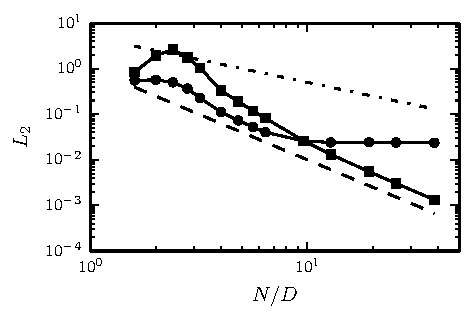
\includegraphics[width=0.6\textwidth]{figs/plot.pdf}
  \caption{This is a figure of some data.}
  \label{fig:plot}
\end{figure}

In \LaTeX{} figures may float and move around to a location that is optimized using mathematics. The htbp in the definition of the figure environment means here,top,bottom,page and is the order of preference for where the figure goes.  

Figure~\ref{fig:photo} shows you can also put pictures into \LaTeX{} documents.  The size of the figure is controlled by adjusting width.  If you find your figures are often floating to a page of their own consider changing their size and/or adding more text.

\begin{figure}[htbp]
  \centering
  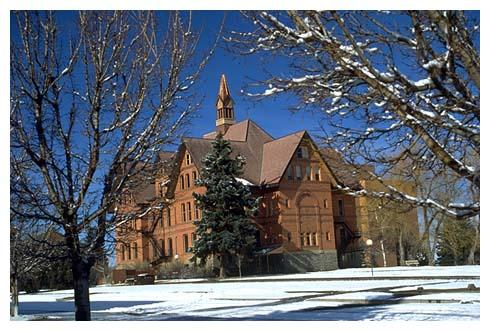
\includegraphics[width=0.6\textwidth]{figs/MSU.jpg}
  \caption{Montana Hall on Montana State University's campus.}
  \label{fig:photo}
\end{figure}

Figure~\ref{fig:tikz} shows that you can create figures directly within your \LaTeX{} document using, for example, the tikz package.
\begin{figure}[htbp]
  \centering
  % Define spring
  \tikzstyle{spring}=[thick,decorate,decoration={zigzag,pre length=0.75cm,post length=0.75cm,segment length=4}]
  \begin{tikzpicture}[scale=2.5]
    % Draw wall
    \draw [] (1,0) -- (1,2);
    \foreach \y in {0,0.2,...,2.1}{
      \draw [] (1,\y) -- ++(-0.25,-0.25);
    }
    % Draw springs
    \foreach \x in {1,...,3} {
      \draw [spring] (\x,1) -- node[pos=0.5,below]{$k_{\x}$} (\x+1,1);
    }
    % Draw nodes and labels
    \foreach \x in {1,...,4} {
      \fill (\x,1) circle (0.07cm);
      \node [below right=0.03cm] at (\x,1) {$\x$};
      \draw (\x,1) -- (\x,1.5);
      \draw [arrows=-latex] (\x,1.25) -- node[pos=1,above]{$F_{\x}$} (\x+0.4,1.25);
    }
    % Draw axis
    \draw [arrows=-latex] (1,0) -- node[pos=1,above]{$x$}(5,0);
  \end{tikzpicture}
  \caption{Figure created using the tikz package.}
  \label{fig:tikz}
\end{figure}


\section{Tables}\label{Sect:tabs}
Tables can be created directly in your \LaTeX{} document.  Table~\ref{tab:ice} shows how a short caption can be used in the table of contents and a long caption in the figure.  In the table of contents ``Area of ice sheet'' is listed above the table ``Area of ice sheet in millions of square miles with time.'' is listed.  This is done by adding an optional argument to the \verb|\caption| command, \ie, \verb|\caption[Short Caption]{Long Caption}|.

\begin{table}[htbp]
  \centering
  \caption[Area of ice sheet]{Area of ice sheet in millions of square miles with time.}
  \label{tab:ice}
  \begin{tabular}{c | ccccccc}
    Year  & 1985 & 1990 & 1995 & 2000 & 2005 & 2010 & 2015\\\hline
    Area  & 16.2 & 15.5   & 15.2  & 15.5  & 14.6 & 15.4 & 14.5 
  \end{tabular}
\end{table}

\section{References and Citations}\label{Sect:ref_cite}

\subsection{Referencing other parts of the document}\label{Sect:ref}
Equations, figures, tables, sections, and chapters can be references using the \verb|\ref{label}| command.  For example, \verb|\ref{fig:plot}| references Fig.~\ref{fig:plot}.  

You can also use the \verb|\vref| command to also get the page number.  For example, \verb|\vref{fig:plot}| references Fig.~\vref{fig:plot}.

The \verb|label| used in the \verb|\ref| command can be anything you want to use. It is helpful to use a convention.  For example, all figures could have a label that starts with \verb|fig:| and all table labels could start with \verb|tab:|.

\subsection{Citing others work}\label{Sect:cite}
Citing others work is an important aspect of all scientific writing.  All citations should be placed in the .bib file(s) listed in your main.tex document.  Cite others work using the \verb|\cite| command, \eg,~\cite{owkes_mesh-decoupled_2015}.  Multiple citations should be done within one cite command, \eg,~\cite{desjardins_direct_2013,owkes_discontinuous_2013,owkes_computational_2014}.  





% This chapter shows how to include a manuscript as a chapter in your thesis or dissertation
% if you are using the manuscript option http://www.montana.edu/etd/format_manuscript.html

\chapter{Title of manuscript you are\\ including as a chapter}\label{CH:manuscript}

\section{Contribution of Authors and Co-Authors}

\noindent Manuscript in following chapter
% Manuscript in Chapter~\ref{CH:manuscript}  % Use this option if using altchapter (numbered chapters and sections)

\noindent Author: [type author name here]

\begin{singlespace}
  \noindent Contributions: [list contributions here, single-spaced]
\end{singlespace}

\noindent Co-Author: [type author name here]

\begin{singlespace}
  \noindent Contributions: [list contributions here, single-spaced]
\end{singlespace}

\noindent Co-Author: [type author name here]

\begin{singlespace}
  \noindent Contributions: [list contributions here, single-spaced]
\end{singlespace}

% Make sure you include all authors and co-authors on this page, individually,
% and a brief paragraph of what each has contributed.

\newpage

\section{Manuscript Information}

\noindent [Type Author and Co-author(s) Names Here]

\noindent [Type name of journal here]

\begin{singlespace}
  \noindent Status of Manuscript: \\ % Put an x in one of the options below
  \underline{\phantom{~~X~~}} Prepared for submission to a peer-reviewed journal\\
  \underline{\phantom{~~X~~}} Officially submitted to a peer-reviewed journal\\
  \underline{~~X~~} Accepted by a peer-reviewed journal\\
  \underline{\phantom{~~X~~}} Published in a peer-reviewed journal
\end{singlespace}

\begin{singlespace}
  \noindent [Type name of publisher here]\\
  [Type date of submission here]\\ % submitted manuscript – otherwise leave blank
  [Type date the manuscript will appear here] \\ % accepted work – otherwise leave blank
  [Type issue in which manuscript appears here] \\ % published work – otherwise leave blank)
  [Type DOI, if available]
\end{singlespace}



\chapter{Conclusion}\label{conclusion}

\LaTeX{} produces documents that look great, automatically handles references and citations, and easily incorporates figures and tables.  This is not a guide to \LaTeX{} but rather an introduction to the MSU style.  If you want more information about \LaTeX{} many introductory guides can be found online.
% Add additional chapters here

% REFERENCES
% Uncomment to use natbib instead of biblatex
% \bibliography{mybib} % Bibliography.  Add your .bib file(s) here
% \bibliographystyle{plainnat} % Use a style you and your adviser like
% \references  % Reference title and TOC entry

% TODO: "REFERENCES" shows up in all caps in the pdf bookmarks, whereas when using bibtex that was not the case. Other than that, it looks like the formatting is okay when using biblatex instead of bibtex...
% TODO: Support using biblatex when there are appendices (REFERENCES CITED needs to be on a separate page in this case).
% Comment out to use natbib instead of biblatex
% NOTE: the vskip in the prenote makes it so there is a triple space between the heading and the first bib entry.
% NOTE: singlespacing ensures that each entry is single-spaced, while the space between entries is double-spaced.
\singlespacing{
    \printbibliography[prenote={\vskip 0pt}, heading=bibintoc, title={REFERENCES CITED}]
}

% APPENDIX
% If you have an appendix use either the option appendsingle (1 appendix) or appendmultiple (>1 appendix) in your document class
% If you do not have an appendix comment out below and remove the appendsingle/multiple option from the document class
\appendix
\chapter{Example Code}\label{appendixa}
This work used the following MATLAB code to produce basically nothing.  But, I'll include it here for the sake of an example.
\begin{lstlisting}
% MATLAB code to say `hello world'
disp(`Hello world')
\end{lstlisting}


%\chapter{Example Schematic}\label{appendixb}
\begin{sidewaysfigure}[ht!]
  \centering
  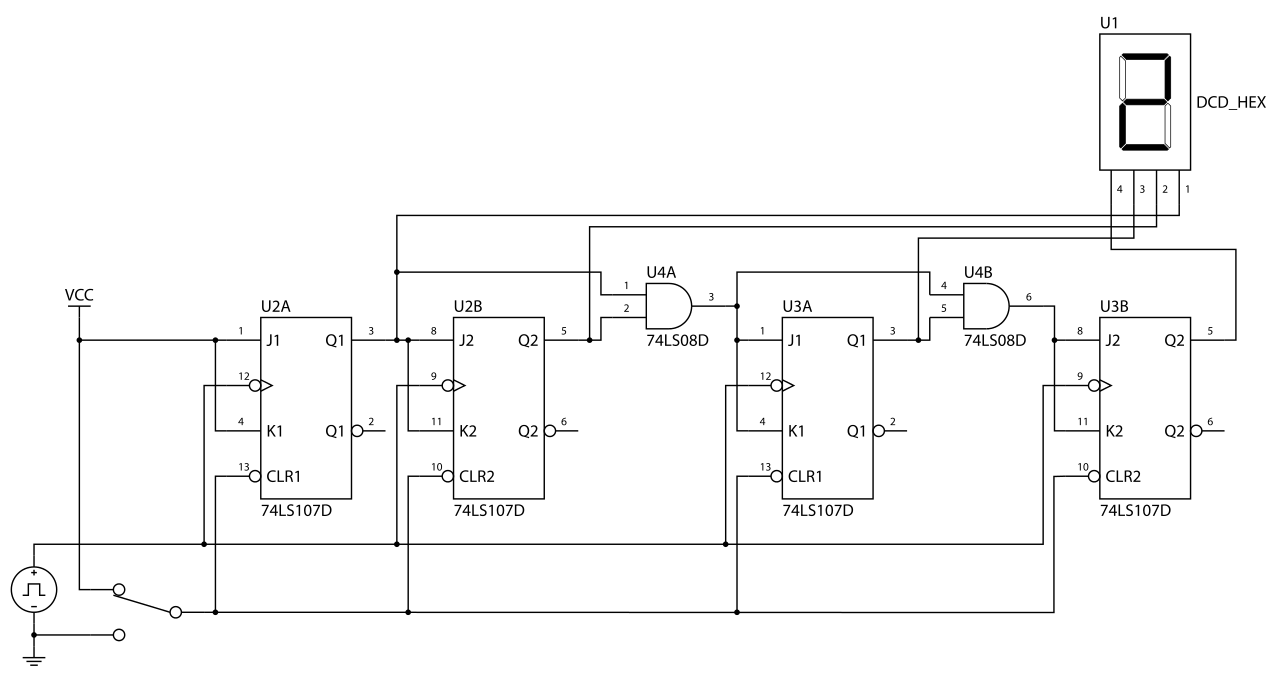
\includegraphics[width=\textheight]{figs/schematic.png}
  \caption{Large schematic on landscape page}
  \label{fig:sche}
\end{sidewaysfigure}


\end{document}
% do not put anything after this

